\chapter{Marco Teórico}

\subsection{¿Qué es el expediente clínico electrónico?}

Con el avance de las ciencias y la tecnología, este concepto evoluciona, considerándose como un “Sistema Informático que almacena los datos del paciente en formato digital, que se almacenan e intercambian de manera segura y puede ser accesado por múltiples usuarios autorizados. Contiene información retrospectiva, concurrente y prospectiva y su principal propósito es soportar de manera continua, eficiente, con calidad e integral la atención y cuidados de salud”. \cite{marco1}
El expediente clínico electrónico
En México existe una norma oficial del expediente clínico (NOM-168-SSA1-1998), la cual fue emitida en el año de 1998 y posteriormente modificada en el año 2003 para que incluyera y validara la posibilidad de la existencia de un expediente clínico electrónico. Por lo tanto, la norma del expediente clínico mexicano, debe ser la base para la creación de un expediente clínico electrónico estándar para todo México. Además, dicha norma se complementa con otras normas como lo son:
\begin{itemize}
  \item NOM-003-SSA2-1993. Para la disposición de sangre humana y sus componentes con fines terapéuticos.
  \item NOM-005-SSA2-1993. De los servicios de planificación familiar.
  \item NOM-006-SSA2-1993. Para la prevención y control de la tuberculosis en la atención primaria a la salud.
  \item NOM-007-SSA2-1993. Atención a la mujer durante el embarazo, parto y puerperio y del recién Nacido.
  \item NOM-008-SSA2-1993. Control de la nutrición, crecimiento y desarrollo del niño y del adolescente.
  \item NOM-013-SSA2-1994. Para la prevención y control de enfermedades bucales.
  \item NOM-014-SSA2-1994. Para la prevención, tratamiento y control del cáncer del útero y de mama en la atención primaria.
  \item NOM-015-SSA2-1994. Para la prevención, tratamiento y control de la diabetes mellitus en la atención primaria.
  \item NOM-017-SSA2-1994. Para la vigilancia epidemiológica.
  \item NOM-024-SSA2-1994. Para la prevención y control de las infecciones respiratorias agudas.
  \item NOM-025-SSA2-1994. Para la prestación de servicios de salud en unidades de atención integral hospitalaria Médico-Psiquiátrica. \cite{marco2}

\end{itemize}

\subsection{Estándares y protocolos}

La existencia y eficiencia de ECE universal exige en consecuencia la adopción de un lenguaje estandarizado: médico, clínico y de comunicaciones. A continuación, se describen algunos de los estándares más relevantes a considerar:
\begin{itemize}
  \item CIE (Clasificación estadística internacional de enfermedades y problemas de salud). Esta clasificación es constantemente actualizada por la Organización Mundial de la Salud (OMS). Por mucho, la versión más estandarizada de esta clasificación es la versión 9, sin embargo, esta versión de la CIE se encuentra obsoleta, puesto que data de los años 70. En México y en países como Estados Unidos se sigue usando dicha versión de clasificación en los sistemas de gestión hospitalaria, en muchos casos por el costo que implica el cambio a la nueva versión. En México, el cambio a las nuevas versiones de la clasificación CIE implica un costo mucho menor que en los países más avanzados, dada la escasa penetración de los sistemas de gestión hospitalaria integrales. \cite{marco2}

  \item SNOMEDCT (Systematized Nomenclature of MedicineClinical Terms). Esta nomenclatura de términos médicos y clínicos fue desarrollada en USA con la finalidad de establecerla como un lenguaje médico universal; es de mayor alcance en temas y dimensiones que la CIE, ya que abarca no solo enfermedades, también procedimientos y otros aspectos clínicos y médicos. De hecho, aunque SNOMED CT fue desarrollada independientemente de la CIE, se han creado tablas de cruce entre ambas clasificaciones. En México predomina el uso de la clasificación CIE, sin embargo, la cercanía y relación estrecha con los Estados Unidos de América podría en un futuro motivar al uso también1 de la clasificación SNOMED CT. \cite{marco2}
  \item HL7 (Health Level Seven International). HL7 es un estándar orientado al formato de los datos e intercambio de información entre diferentes sistemas de información de salud o gestión hospitalaria. Estándares como la clasificación CIE o la nomenclatura SNOMED CT establecen el lenguaje medico y clínico, pero HL7 establece los mecanismos de transporte de la información médica recolectada en forma de expedientes clínicos, estadísticas, entre otros. Además, HL7 permite la interoperabilidad entre los diferentes sistemas de gestión hospitalaria públicos y privados. Por ejemplo, si la Secretaria de Salud solicitará a los hospitales públicos y privados información estadística sobre la proliferación de ciertas enfermedades, una manera de estandarizar las transmisiones de dicha información sería mediante el protocolo HL7. \cite{marco2}
  \item DICM (Digital Imaging and Communication in Medicine). DICOM es un estándar diseñado para el manejo, almacenamiento, impresión y transmisión de imágenes médicas que deben ser incluidas en el expediente clínico electrónico. La imagenología es un área importante en el diagnóstico, prevención y seguimiento de enfermedades o padecimientos, por lo que su inclusión en el expediente clínico electrónico es relevante.\cite{marco2}
  \item CRIPTOGRAFÍA. La criptografía es la ciencia que versa sobre el cifrado de información con fines de seguridad y confidencialidad. Es un área tan dinámica que sería difícil mencionar un estándar que el día de mañana no sea remplazado rápidamente o que carezca de vulnerabilidades. Sin embargo, en un contexto comparativo, un sistema de gestión hospitalaria electrónico en línea requiere de un nivel de seguridad informática similar al usado en la banca electrónica.
\end{itemize}

Actualmente el protocolo de seguridad más usado en la banca electrónica es el SHTTP (Secure Hyper Text Transfer Protocol), que, en combinación con otras medidas de seguridad (llaves electrónicas, firewalls, etc.), garantiza al usuario “cierto nivel de certeza” de que sus datos personales y dinero se encuentran seguros. Este nivel de seguridad es deseable también en los sistemas de gestión hospitalaria masivos ya que tanto la población, como los profesionales de la salud, guardan dudas razonables respecto de la seguridad de la información. \cite{marco2}
\subsection{Aspectos legales}
A pesar de que la norma del expediente clínico contempla la grabación del expediente en medios electrónicos aún no existe una norma o ley que regule de manera cabal el uso del expediente clínico electrónico. De hecho, en México, el marco jurídico para estos aspectos aún no se desarrolla de manera adecuada. Sin embargo, el estado de Colima es la excepción, ya que actualmente cuenta una ley de protección de datos personales, que por ser general aplica a diversos ámbitos. Sin embargo, a continuación, se presenta algunos artículos que pueden afectar el uso del expediente clínico electrónico:
\begin{itemize}
  \item El Artículo 4, fracción XI menciona que: “Los servidores públicos, profesionales, trabajadores y otras personas que por razón de sus actividades tengan acceso a archivos o datos de carácter personal, estarán obligados a mantener la confidencialidad de los mismos y a no darlos a conocer a terceros. Esta obligación subsistirá aun después de finalizar las relaciones que les dieron acceso a los datos. La contravención a esta disposición será sancionada de conformidad con la legislación penal”. Un aspecto que deja abierto a la discusión este punto es: ¿quién exactamente puede o debe tener acceso a la información del expediente clínico? El sentido común dicta que únicamente el médico o los médicos que tratan al paciente deben tener acceso, aunque puede haber excepciones como la extracción de datos para realizar estadísticas. \cite{marco2}
  \item El Artículo 4, fracción XII menciona que: “Los datos personales relativos a la salud podrán ser operados por los profesionales e instituciones de acuerdo con la legislación sanitaria, pero conservando la confidencialidad de los mismos de acuerdo con la presente Ley”. En esta fracción se contempla la posibilidad de que los datos del expediente clínico electrónico sean usados por profesionales e instituciones. Esto es relevante ya que permite que los datos del expediente clínico electrónico se usen no sólo para el tratamiento personalizado de cada paciente, también para generar estadísticas y alertas sanitarias, modelado de enfermedades, entre otros aspectos.\cite{marco2}
  \item El Artículo 5º menciona que: “El responsable del archivo deberá establecer los mecanismos de seguridad que garanticen la confiabilidad y confidencialidad de los datos. El reglamento correspondiente establecerá las características mínimas de seguridad que deban tenerse en las instalaciones que manejen datos de carácter personal”. Este artículo establece que debe existir una protección de la información y que esta será establecida en un reglamento que debe ser creado, en este caso, por la Secretaria de Salud. \cite{marco2}
  \item El Artículo 7º menciona que: “Las personas físicas o morales cuyos datos de carácter personal hayan sido integrados a un archivo, tendrán los siguientes derechos […] solicitar y obtener gratuitamente información de sus datos de carácter personal y del origen de esos datos”. El artículo 7 establece esencialmente que el paciente podrá recibir una copia “gratuita” al año de su expediente clínico electrónico para los fines que el paciente crea más convenientes; lo que conduce a la siguiente pregunta: ¿quién es el dueño del expediente clínico electrónico?
  \item ¿Es propiedad del médico, del hospital, del estado o del paciente? En algunos países se establece que el paciente es el dueño del expediente clínico electrónico, dándole mayor poder y responsabilidades al paciente sobre su expediente. Por ejemplo, se puede permitir que el paciente haga anotaciones sobre su estado de salud, consumo de medicamentos no controlados, alergias, exposición a sustancias, hábitos y otros aspectos que hasta ahora son normalmente una incógnita y que pueden resultar relevantes en los tratamientos médicos. \cite{marco2}

\end{itemize}

\subsection{El Desarrollo de un expediente clínico electrónico}

 Para desarrollar una aplicación con estas características hay una gran cantidad de métodos y tecnologías que podríamos implementar. Ejemplo de ello son los frameworks para el desarrollo web, para poder entender mejor “con el término framework, nos estamos refiriendo a una estructura software compuesta de componentes personalizables e intercambiables para el desarrollo de una aplicación. En otras palabras, un framework se puede considerar como una aplicación genérica incompleta y configurable a la que podemos añadirle las últimas piezas para construir una aplicación concreta.” (Gutiérrez Javier, s.f).
Pero para poder comprender aún más como funciona un framwork es necesario saber que es el MVC (Modelo – Vista – Controlador).
\subsubsection{Por qué MVC}

La rama de la ingeniería del software se preocupa por crear procesos que aseguren calidad en los programas que se realizan y esa calidad atiende a diversos parámetros que son deseables para todo desarrollo, como la estructuración de los programas o reutilización del código, lo que debe influir positivamente en la facilidad de desarrollo y el mantenimiento.
Los ingenieros del software se dedican a estudiar de qué manera se pueden mejorar los procesos de creación de software y una de las soluciones a las que han llegado es la arquitectura basada en capas que separan el código en función de sus responsabilidades o conceptos. Por tanto, cuando estudiamos MVC lo primero que tenemos que saber es que está ahí para ayudarnos a crear aplicaciones con mayor calidad. \cite{marco3}

\subsection{Modelos}

Es la capa donde se trabaja con los datos, por tanto, contendrá mecanismos para acceder a la información y también para actualizar su estado. Los datos los tendremos habitualmente en una base de datos, por lo que en los modelos tendremos todas las funciones que accederán a las tablas y harán los correspondientes selects, updates, inserts, etc.
No obstante, cabe mencionar que cuando se trabaja con MCV lo habitual también es utilizar otras librerías como PDO o algún ORM como Doctrine, que nos permiten trabajar con abstracción de bases de datos y persistencia en objetos. Por ello, en vez de usar directamente sentencias SQL, que suelen depender del motor de base de datos con el que se esté trabajando, se utiliza un dialecto de acceso a datos basado en clases y objetos. \cite{marco3}


\subsection{Vistas}
Las vistas, como su nombre nos hacen entender, contienen el código de nuestra aplicación que va a producir la visualización de las interfaces de usuario, o sea, el código que nos permitirá renderizar los estados de nuestra aplicación en HTML. En las vistas nada más tenemos los códigos HTML y PHP que nos permite mostrar la salida.
En la vista generalmente trabajamos con los datos, sin embargo, no se realiza un acceso directo a éstos. Las vistas requerirán los datos a los modelos y ellas se generará la salida, tal como nuestra aplicación requiera. \cite{marco3}

\subsection{Controladores}
Contiene el código necesario para responder a las acciones que se solicitan en la aplicación, como visualizar un elemento, realizar una compra, una búsqueda de información, etc.
En realidad, es una capa que sirve de enlace entre las vistas y los modelos, respondiendo a los mecanismos que puedan requerirse para implementar las necesidades de nuestra aplicación. Sin embargo, su responsabilidad no es manipular directamente datos, ni mostrar ningún tipo de salida, sino servir de enlace entre los modelos y las vistas para implementar las diversas necesidades del desarrollo. \cite{marco3} \ref{figura8}
\begin{figure}[h]
  \label{figura8}
  \centering
  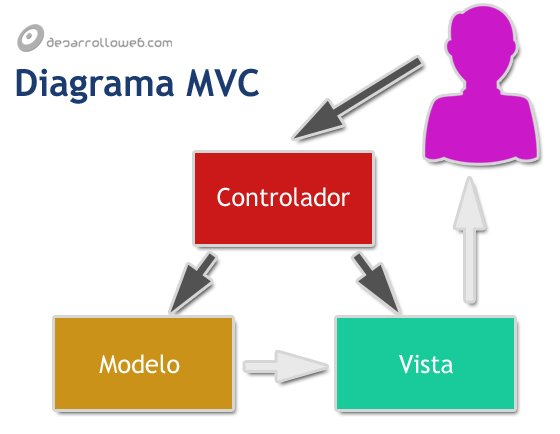
\includegraphics[scale=.35]{lib/assets/8}
  \caption{Diagrama MVC.}
\end{figure}





\subsection{Angular}
Framework de desarrollo.
Angular es una herramienta de desarrollo creada por Google, cuyo objetivo es facilitar el manejo de grandes proyectos, el paradigma de programación utilizado es orientado a componentes, lo cual hace que cada componente se pueda reutilizar en distintas áreas del proyecto, ahorrando así grandes cantidades de código y por su puesto manejar proyectos de gran tamaño con mayor eficacia. Angular cuenta con una serie de herramientas que la colocan a la altura de los mejores frameworks de desarrollo web y aplicaciones móvil.  Ejemplo de ellas: \cite{Angular} \ref{figura9}
\begin{figure}[h]
  \label{figura9}
  \centering
  
\includegraphics[scale=.70]{lib/assets/9}
  \caption{Logo de Angular.}
\end{figure}



\subsection{TypeScript}
Es un superset (superconjunto) de JavaScript de código abierto, el cual está desarrollado por Microsoft. Está diseñado para utilizarse en su desarrollo la programación orientada a objetos(POO). Lo cual ayuda en el manejo de grandes cantidades de código en proyectos con gran escalabilidad. Haciendo de typeScrip un gran aliado al desarrollar en Angular,hoy en día es el lenguaje que mejor interacción tiene con este framework, además cuenta con una vasta documentación. \cite{typeScript} \ref{figura10}
\begin{figure}[h]
  \label{figura10}
  \centering
  
\includegraphics[scale=.35]{lib/assets/10}
  \caption{Logo de TypeScript}
\end{figure}



\subsection{Bulma}
Bulma es un Framework CSS basado en flexbox, además es totalmente responsivo lo cual significa que se adapta el diseño a el tamaño de la pantalla, modular y la documentación es sumamente extensa en su página oficial.
Las líneas de diseño de Material Design, propuesta por Google en junio del 2014, son tomadas en Bulma, lo cual tener unas líneas de diseño bien marcadas, facilita a que todo el entorno de la aplicación web sea homogéneo.\cite{Bulma} \ref{figura11}
\begin{figure}[h]
  \label{figura11}
  \centering
  
\includegraphics[scale=1]{lib/assets/11}
  \caption{Logo de Bulma.}
\end{figure}


\subsection{MySQL}
MySQL es la base de datos de código abierto número uno del mundo, es la base de datos número uno para Web y es una excelente base de datos embebida. Más de 3.000 ISVs y OEMs, incluyendo 8 de los 10 mayores, y 17 de los 20 principales proveedores de software de todo el mundo confían en MySQL como base de datos de sus productos.
La gran documentación de MySQL la hace una de las bases de datos más utilizadas en el mundo y además cuenta con una gran comunidad lo cual es de gran ayuda para solucionar problemáticas cotidianas al desarrollar aplicaciones web que interactúan con bases de datos relacionales.
El software MySQL ™ ofrece una, multi-threaded, multi-usuario muy rápido, robusto y SQL (Structured Query Language) del servidor de base de datos. Servidor MySQL está diseñado para sistemas de producción de misión crítica, carga pesada, así como para integrarse en software para ser distribuido. \cite{mysql} \ref{figura12}
\begin{figure}[h]
  \label{figura12}
  \centering
  
\includegraphics[scale=1]{lib/assets/12}
  \caption{Logo de MySQL.}
\end{figure}


Fig 10.
